%----------------------------------------------------------
\chapter{Программная реализация}
\label{ch:chap3_soft_architecture}
%----------------------------------------------------------
\section{Архитектура}
\label{sec:architecture}

В структуре программы почти любого компилятора можно выделить следующие части:

\begin{figure}[H]
    \centering
    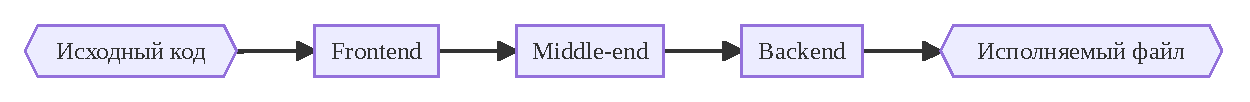
\includegraphics[width=\textwidth]{figures/.generated/arch}
    \caption{Архитектура большинства современных компиляторов}
    \label{fig:arch}
\end{figure}

Сопоставляя эти части с рис. \ref{fig:pipeline} можно прийти к такому выводу:
\begin{inparaenum}[1)]
    \item к frontend части относятся лексический и синтаксический анализ,
    \item к middle-end части - семантический анализ и генерация промежуточного представления,
    \item к backend части - генерация машинного кода.
\end{inparaenum}
Разработка frontend части была завершена ещё до этой работы и не будет подробно раскрываться.

Проект разрабатывается с использованием языка программирования Rust.
Этот язык предлагает надежный концепт управления памятью, не имея при этом сборщика мусора \cite{RustMemory}.
Кроме того, он соперничает по скорости с C и C++ и применяется в довольно широком спектре приложений.
Основные преимущества выбора этого языка:
\begin{itemize}
    \item Rust работает быстрее за счёт использования мощных оптимизаторов, а так же применяет более строгие требования к разработке в целом,
    \item он предоставляет больше гарантий разработчику, как посредством его системы типов, так и другими средствами, например, borrow checker,
    \item система сборки создает нативный файл программы - его можно запустить, не имея на машине специальных сред выполнения.
\end{itemize}

Работать с большими проектами в разы удобнее и эффективнее при грамотном разбиении на модули.
В экосистеме Rust такие модули именуются крейтами (англ. crates).
На диаграмме ниже представлено разбиение на модули проекта Kodept.
При этом сплошной линией выделено отношение модулей (от независимых к зависимым), пунктирной линией отмечена передача данных во время работы программы (от начала к концу).
Под диагностиками необходимо понимать сообщения компилятора об исходной программе.

\begin{figure}[H]
    \centering
    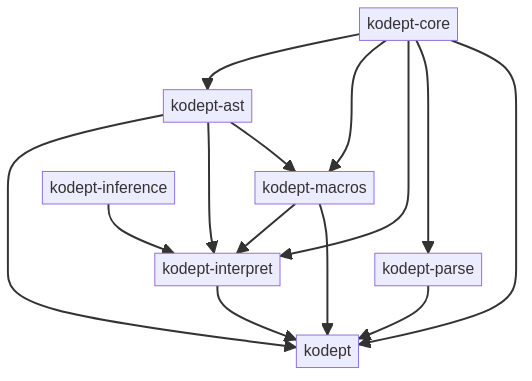
\includegraphics[width=\textwidth]{figures/.generated/modules}
    \caption{Иерархия модулей в проекте}
    \label{fig:modules}
\end{figure}

В рамках этой работы внимание будет сконцентрировано вокруг модулей \lstinline{kodept-ast}, \lstinline{kodept-interpret} и \lstinline{kodept-inference}.
Однако, дадим кратное описание остальных модулей:
\begin{itemize}
    \item \lstinline{kodept-core} отвечает за определение основных структур данных, необходимых в остальных частях приложения, в частности, в нем определена структура \textit{дерева разбора},
    \item \lstinline{kodept-parse} отвечает за лексический и синтаксический анализ, определяя набор синтаксических анализаторов (парсеров), которые генерируют дерево разбора,
    \item \lstinline{kodept-macros} нужен для работы с AST и создания диагностик,
    \item \lstinline{kodept} является корневым модулем и обеспечивает запуск стадий компилятора для входных файлов.
\end{itemize}

Дерево разбора - подробная версия AST, куда включается вся информация, полученная от парсеров.
Нужно для восстановления конкретной точки в исходном коде при создании диагностики.

В модуле \lstinline{kodept-ast} определена структура AST и его хранения.
Рассмотрим некоторые проблемы, возникшие при проектировании этого модуля.

\section{Проблема хранения абстрактного синтаксического дерева}
\label{sec:ast_structure}

Обычно структура AST реализована в программе в виде вложенных друг в друга структур с данными, описывающими тот или иной синтаксис языка (листинг~\ref{lst:ast_node}).

\begin{lstlisting}[language=C, label=lst:ast_node, caption={Псевдокод структур, представляющей собой описание синтаксиса функции в языке программирования.}]
    struct Function {
        vector<Parameter> parameters;
        Type return_type;
        Statement body;
    }
    struct Parameter {
        string name;
        Type type;
    }
    struct Type {
        string identifier;
    }
    struct Statement {
        // ...
    }
\end{lstlisting}

Однако при таком подходе возникают определенные трудности.
Чтобы написать обход AST, необходимо использовать исключительно рекурсивную реализацию.
Это может стать проблемой при формировании большого AST, что его обход приведет к переполнению стека.
Кроме того, гораздо большее неудобство возникает и при непосредственно реализации: нужно добавить по отдельной функции обхода для каждого узла дерева.
При добавлении нового синтаксиса править код придется сразу в нескольких местах, а это усложняет поддерживаемость.

Поэтому необходимо было придумать более оптимизированный вариант для хранения AST.
В итоге было решено переписать имеющиеся структуры так, чтобы они включали только те данные, которые непосредственно относятся к ним, а также включали цифровой идентификатор.

\begin{lstlisting}[language=C, label=lst:ast_node_after, caption={Псевдокод структур после преобразования.}]
    struct Function {
        int id;
    }
    struct Parameter {
        string name;
        int id;
    }
    struct Type {
        string identifier;
        int id;
    }
    struct Statement {
        // ...
        int id;
    }
\end{lstlisting}

Такая композиция позволяет хранить все объекты этих структур в одном месте, линейно.
А с помощью индексов моделировать между ними взаимосвязь.
Проще говоря, все свелось к хранению обычного графа, где вершины - идентификаторы.
С таким видом гораздо удобнее работать, так как алгоритм перебора оперирует числами.
Также хранение небольших структур в одном месте повышает вероятность попадания в кеш-память.

При применении <<графового>> хранения нарушается непосредственная взаимосвязь между структурами.
Таким образом, становится непонятно, какие структуры могут быть в каких изначально были <<вложены>>.
Но это легко решается с помощью системы типов Rust.
А именно: вводятся так называемые свойства принадлежности.
Например, функция в качестве вложенных данных могла иметь вектор параметров, возвращаемый тип и тело.
Значит, структура Parameter может выступать в качестве <<ребенка>> структуры Function.
Также в структуру Function добавляются методы для доступа к объявленным <<детям>>.
Таким образом сохраняется безопасность при работе с AST.

\begin{lstlisting}[label=lst:node, caption={Упрощенное представление структур после всех доработок на языке Rust}]
    struct Function {
        id: usize
    }

    struct Parameter {
        id: usize,
        name: string
    }

    impl HasChildrenMarker<Vec<Parameter>> for Function {
        // ...
    }

    impl Function {
        fn parameters(&self, /* ... */) -> Vec<&Parameter> {
            // ...
        }
    }
\end{lstlisting}

Для наглядного изучения AST, было добавлено сохранение дерева в файл формата DOT~\cite{Dot}.
В вершинах графа расположены имена синтаксических конструкций и числовой идентификатор.
В ребрах - специальный тег, призванный отличать одни вершины от других.
На рисунке~\ref{fig:ast_dot} изображена визуализация AST программы с листинга~\ref{lst:kodept}.

\section{Организация доступа к элементам абстрактного синтаксического дерева}
\label{sec:ast_access}

С помощью модуля \lstinline{kodept-macros} организовывается анализ AST\@.
Во время этого элементы, составляющие дерево, могут быть изменены.
К сожалению, из-за специфики Rust, в момент времени может существовать только 1 ссылка на объект, допускающая изменение (exclusive mutable access).
Иногда разработчику не обойтись без разделяемого изменяемого состояния.
Для этого прибегают к использованию внутренней изменяемости (англ. interior mutability).

Interior mutability позволяет изменять внутренние данные неизменяемой структуры.
Самым популярным способом является использование указателя с подсчетом ссылок (reference-counted pointer, RC) вкупе с проверкой заимствований во время выполнения (RefCell).
Аналогом из C++ можно считать использование shared\_ptr.

\begin{lstlisting}[label=lst:interior, caption={Упрощенная реализация структур Rc и RefCell на псевдокоде}]
    struct Rc<T> {
        int strong_count;
        int weak_count;
        T data;
    }

    struct RefCell<T> {
        T data;
        int borrows_count;
    }
\end{lstlisting}

При анализе AST элементы могут поменяться, а структура - нет.
Получается, что граф - неизменяемая структура, но его внутренние данные изменяемы.
Это как раз подходит под понятие interior mutability.
Но использование проверок во время выполнения, а также хранение дополнительных счетчиков для RC плохо влияет на производительность и использование памяти.

Предлагается использовать вместо привычной комбинации из RC + RefCell \textit{zero-cost} абстракцию GhostCell~\cite{GhostCell}.
Термином zero-cost или <<нулевых затрат>> называют полное отсутствие затрат во время выполнения - все необходимые преобразования выполняет компилятор во время компиляции.
Основной идеей GhostCell является разделение ответственности за хранение и модификацию данных.
Вводится специальный токен, который дает право изменять данные.

\section{Реализация алгоритма W}
\label{sec:algorithm_W}

За реализацию алгоритма отвечает модуль \lstinline{kodept-inference}.
В нем также находится определение необходимых термов и типов.
Согласно рисунку~\ref{fig:modules}, этот модуль не зависит ни от каких других.
Система типов и алгоритм вывода могут быть определены, используя собственную модель.
Таким образом, достаточно реализовать функцию по конвертации элементов AST в элементы модели.

\subsection{Анализ областей видимости}
\label{subsec:scope_analysis}

Задачей этого анализа является разбиение AST на области видимости (англ. scopes), при этом строится так называемое дерево областей.
Оно состоит из идентификаторов узлов AST, где каждый такой узел начинает новую область.
Внутри области можно найти все объявленные переменные и функции, и удостовериться, что не используются необъявленные.

Например, для программы с листинга~\ref{lst:kodept}, дерево областей будет таким:

\begin{figure}
    \centering
    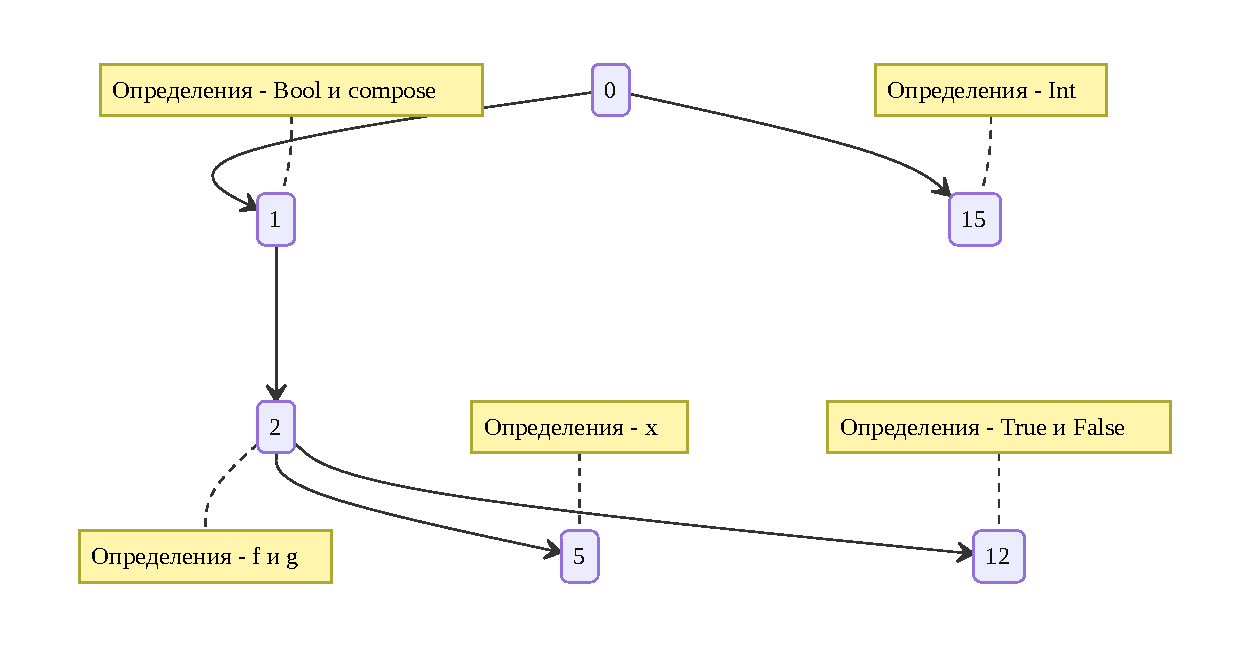
\includegraphics[width=\textwidth]{figures/.generated/scopes}
    \caption{Дерево областей видимости}
    \label{fig:scopes}
\end{figure}

Для каждого определения из любой области можно применить алгоритм W.

В процессе преобразования модели AST (листинг~\ref{lst:nodes}) в термы (\ref{subsec:hindley-milner}), также образуются предположения.
Они играют роль ограничений.
Например, запись \lstinline{val a: Int = expr} добавит предположение $a: Int$.
Таким образом, алгоритм вывода типов проверит, что тип переменной \lstinline{a} совпадает с типом выражения \lstinline{expr}.

%----------------------------------------------------------
